\clearpage
\fancyhead[R]{\sffamily\small\color{Muted}Vulkan / 阴影与探针}
\section{三角形的共边与光照耗时}
神庙的墙由许多三角形拼成。一条光线正好打在两个三角形共用的边上，如果两边都判定光线落在自己外面，光线就会穿过墙。用前后紧挨的两张平面做实验，旧算法的 289 条射线里有 10 条碰到了后面一层。沿着射线把三角形投到二维平面，让两边用相同的计算检查共边，289 条射线就都停在前面。下面把同样的改动放回两个完整场景，看它对阴影和光照计算的影响。

\begin{figure}[H]\centering
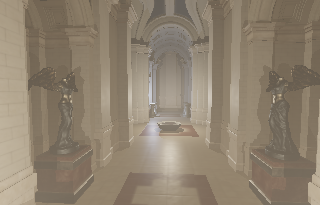
\includegraphics[width=.48\linewidth]{triangle-intersection/Sun-Temple.png}\hfill
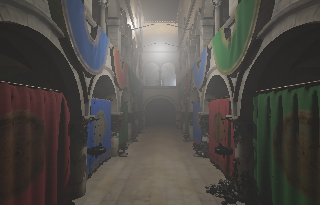
\includegraphics[width=.48\linewidth]{triangle-intersection/Sponza-Atrium.png}
\caption{正式编辑器第 24 帧的场景面板。左边的 Sun Temple 有 606\,376 个三角形和 8 个点光源；右边的 Sponza 有 262\,267 个三角形和 3 个点光源。两图都以 $320\times205$ 像素计算，雾沿视线分八步取样。}
\end{figure}

点光源从墙面朝灯检查遮挡，遇到一块挡光的砖就能返回。探针要找出沿途最近的表面，再读取那里的材质和光照。每帧更新 $12\times6\times7$ 个探针，每个探针朝六个方向取样，每方向两条射线，一共 6\,048 条。把探针照到的光分给屏幕上的像素时，只需读取附近探针，表中单列这一项作对照。

{\smalltable\noindent\begin{tabularx}{\linewidth}{@{}Xrrrr@{}}\toprule
GPU 时间（毫秒）& 逐灯照明 & 更新探针 & 读取探针 & 八步雾\\\midrule
Sun Temple，旧版     & 1.020 & 1.176 & 0.013 & 4.402\\
Sun Temple，共边检查 & 1.607 & 2.259 & 0.012 & 5.723\\
Sun Temple，共边检查与新分组 & 0.790 & 1.472 & 0.011 & 2.554\\\addlinespace
Sponza，旧版        & 0.911 & 1.189 & 0.012 & 3.666\\
Sponza，共边检查    & 1.511 & 2.139 & 0.012 & 4.633\\
Sponza，共边检查与新分组 & 0.795 & 1.035 & 0.012 & 2.571\\\bottomrule
\end{tabularx}\par}

第一次只改共边检查，神庙的探针更新耗时接近翻倍。最终版让一条射线经过的三角形共用一次投影准备，同时改了模型的分组方式。神庙的八步雾比旧版少用 1.848 毫秒，更新探针仍多用 0.296 毫秒；Sponza 的这两项均比旧版快。三版逐灯照明的线性 RGB 完全相同。按每通道 256 级导出最终版和旧版的面板图，神庙只有 8 个像素相差一级，Sponza 有 6 个，两图各有 65\,600 个像素。

使用 RTX 5070 Ti Laptop GPU、Debug x64 编辑器和 RenderDoc 1.47。每份捕获预热一次，再取 11 次 GPU 计时的中位数。表中四项各执行一次；神庙整帧有 70 次绘制、7 次计算，Sponza 有 125 次绘制、6 次计算。

\clearpage
\subsection{神庙模型的包围盒}
从高处看，神庙主体沿一条长廊展开。下图的每个灰点代表落在那一小块地面上方的三角形重心，越黑说明三角形越密。加载模型时，引擎给三角形分组，每组外面套一个能包住它们的长方体，沿分组一层层套下去，就得到一棵包围盒树。一条射线若连外面的盒子都碰不到，里面整组三角形就可以跳过。

\begin{figure}[H]\centering
\panelimage{.48\linewidth}{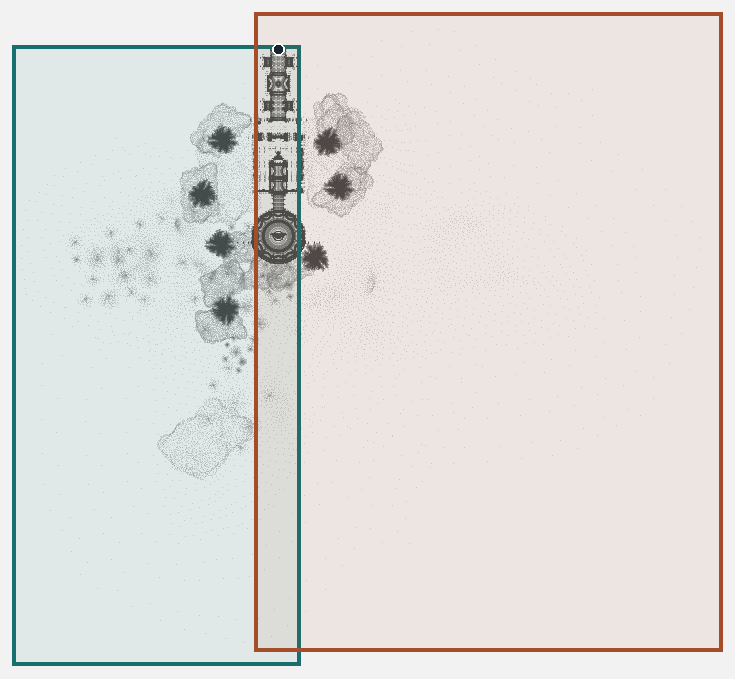
\includegraphics[width=\linewidth]{triangle-intersection/tree-median.png}\\[2pt]

\includegraphics[width=\linewidth]{triangle-intersection/tree-median-entry.png}}{按数量平分 · 每组 303\,188 个三角形}
\hfill
\panelimage{.48\linewidth}{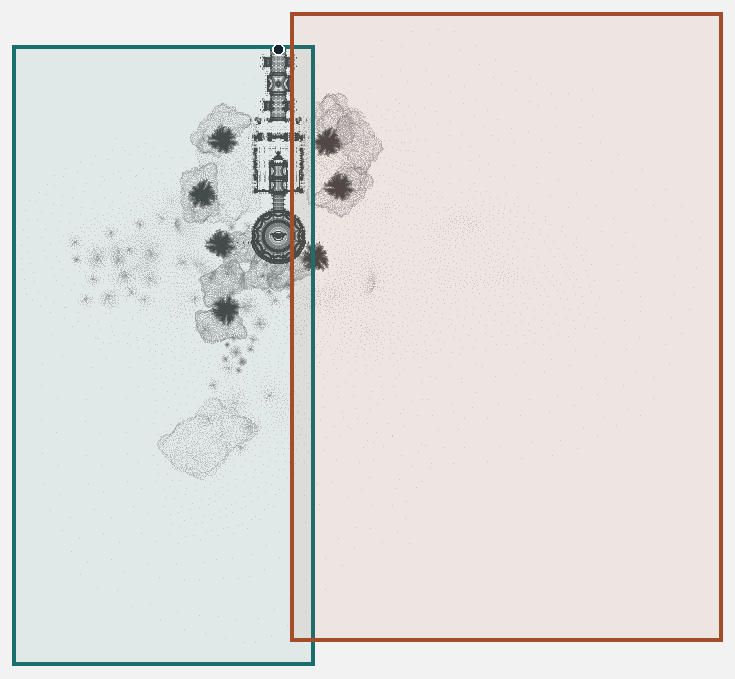
\includegraphics[width=\linewidth]{triangle-intersection/tree-area.png}\\[2pt]

\includegraphics[width=\linewidth]{triangle-intersection/tree-area-entry.png}}{按面积和数量分 · 538\,079 与 68\,297 个}
\caption{上排俯看整座神庙，下排放大长廊入口。青框和棕框是最外层包围盒分出的两组，取自 GPU 收到的节点。黑圆点是上一页的主相机。沿长廊向画面下方看，左图的两个盒子都覆盖了长廊中线，右图的棕框已退到旁边。}
\end{figure}

设一条射线沿长廊中线 $x=0$ 向前走，左右都不偏。左图两个盒子都跨过中线，即使只想查墙面到灯之间有没有遮挡，也可能要继续检查两组。右图把棕框的左边移到 $x=4.76$，这条射线可以跳过整个棕框。青框和棕框在水平方向重叠的宽度从 17.50 个场景单位缩到 9.09 个。图中只画了第一次分组，上一页的 GPU 计时包含整棵树。

从十二段中选一个分界时，引擎估算两边的检查量。把左盒表面积 $A_L$ 乘上它的三角形数 $N_L$，给右盒算同样的量，相加得到 $A_LN_L+A_RN_R$。同一个父盒内，选这个数最小的分界。较大的盒子更有机会被射线碰到，往它里面塞很多三角形，估算的工作就会增加。实现还会先存好每个三角形的包围盒和重心，排好顺序后再移动整份三角形数据。

在 Ryzen 9 8945HX 上交替运行两种建树方法，剔除一对预热后各取五次的中位数。神庙由 5.228 秒变为 3.066 秒，Sponza 由 2.281 秒变为 1.284 秒，耗时从已有三角形开始算到重排完成。每个节点占 48 字节。正式帧中神庙的节点数据从 12.00 降到 11.91\,MiB，Sponza 从 6.00 降到 5.12\,MiB。

\readings{\refitem{https://pbr-book.org/4ed/Primitives_and_Intersection_Acceleration/Bounding_Volume_Hierarchies}{PBRT 第四版 · 包围盒分割成本}\quad
\href{run:../profiling/triangle-intersection/README.md}{捕获、逐次 GPU 读数与 CPU 建树样本}}
